\documentclass[10pt]{report}

\usepackage{float}
\usepackage{graphicx} % do I look like I know what a jpg is?
\usepackage{color}
\usepackage[usenames,dvipsnames,svgnames,table]{xcolor}
%\usepackage{epstopdf}
\usepackage{changepage}
\usepackage{amssymb}
\usepackage{amsthm}
\usepackage{amsmath}
\usepackage{array}
\usepackage{booktabs}
\usepackage{listings}   % Include code snippets
\usepackage{titlesec}
\usepackage{ulem}
\usepackage[linkbordercolor={0.9 .55 .6}]{hyperref}
\usepackage{sfmath}
\usepackage{setspace}
\usepackage{pifont}
\usepackage[toc,page]{appendix}
\usepackage{epigraph}
\pdfpagewidth 8.5in
\pdfpageheight 11in
\topmargin -1.0in
\headheight .75in
\headsep 0in
\textheight 8.75in
\textwidth 7.0in
\oddsidemargin -.25in
\evensidemargin 0in
\footskip .4in
\definecolor{args}{rgb}{0.0,0.05,.33}
\definecolor{mygray}{rgb}{0.5,0.5,0.6}
\definecolor{mybordergray}{rgb}{0.72,0.72,0.85}
\definecolor{mylightblue}{rgb}{.98, .98, 1.00}
\definecolor{mymauve}{rgb}{0.58, 0, 0.82}
\definecolor{mydarkred}{rgb}{0.78, .14, 0}
\lstset{language=C, showstringspaces=false, frame=single, basicstyle=\footnotesize\sffamily, stringstyle=\color{mymauve}, framesep=4pt, xleftmargin=2pt, xrightmargin=2pt, rulecolor=\color{mybordergray}, backgroundcolor=\color{mylightblue},keywordstyle=\color{mydarkred}, commentstyle=\color{mygray}, belowskip=1.5em, aboveskip=1em, tabsize=2, breaklines=true, stepnumber=5, captionpos=t, numbers=left, numbersep=10pt, numberstyle=\tiny\color{mygray}}

\setstretch{1.15}
 
\titleformat*{\subsubsection}{\normalsize\sffamily}



\makeatletter
\def\@makechapterhead#1{%
  \vspace*{50\p@}%
  {\parindent \z@ \raggedright \normalfont
    %\ifnum \c@secnumdepth >\m@ne
    %    \huge\bfseries \@chapapp\space \thechapter
    %    \par\nobreak
    %    \vskip 20\p@
    %\fi
    \interlinepenalty\@M
    \Huge \bfseries #1\par\nobreak
    \vskip 35\p@
  }}
  \makeatother

\newcommand\invisiblechapter[1]{%
	\setcounter{secnumdepth}{0}
  \refstepcounter{chapter}%
  \addcontentsline{toc}{chapter}{\protect #1}%
  \chaptermark{#1}}
  
\long\def\symbolfootnote[#1]#2{\begingroup%
\def\thefootnote{\fnsymbol{footnote}}\footnote[#1]{#2}\endgroup} 


\newcommand{\LFOutADC}[0] {\texttt{LFOutADC}}
\newcommand{\LFOutPin}[0] {\texttt{LFOutPin}}
\newcommand{\errMonADC}[0] {\texttt{errMonADC}}
\newcommand{\errMonPin}[0] {\texttt{errMonPin}}
\newcommand{\coarseDAC}[0] {\texttt{coarseDAC}}
\newcommand{\fineDAC}[0] {\texttt{fineDAC}}
\newcommand{\coarseDACOut}[0] {\texttt{coarseDACOut}}
\newcommand{\fineDACOut}[0] {\texttt{fineDACOut}}
\newcommand{\aPin}[0] {\texttt{aPin}}
\newcommand{\bPin}[0] {\texttt{bPin}}
\newcommand{\blockLockPin}[0] {\texttt{blockLockPin}}
\newcommand{\calibratePin}[0] {\texttt{calibratePin}}
\newcommand{\sampleErrorMonitor}[0] {\texttt{sampleErrorMonitor}}
\newcommand{\greenLEDName}[0] {\textit{Normal Operation}}
\newcommand{\yellowLEDName}[0] {\textit{Calibrating}}
\newcommand{\orangeLEDName}[0] {\textit{Relocking}}
\newcommand{\redLEDName}[0] {\textit{Check System}}



\begin{document}
\begin{titlepage}
	\begin{center}
	\vspace{45mm} %does nothing
	\hspace{17mm}
 % 	\includegraphics[width=100mm]{images/cover.jpg}\newline\\
  	
  	\vspace{20mm}
	\textsc{\Large The University of Colorado Boulder's \\ \vspace{5mm} \huge  Thompson Lab}\\[18mm]
	
	\hspace{20mm}
	\includegraphics[width=80mm]{includes/salamander.png}\newline\\\vspace{20mm}
	\hrule \vspace{4mm}
	{ \huge \bfseries Relocker User Manual}\\[0.4cm]
	\hrule

	\vspace{10mm} \large
	Author List: \\
	Denton Wu (\texttt{dwu2412@gmail.com}) \\
	Graham Greve (\texttt{graham.greve@colorado.edu}) \\
	\vfill

	% Bottom of the page
	{Last Edited: \today}
	\end{center}
\end{titlepage}
\cleardoublepage
\tableofcontents
\cleardoublepage


%%%%%%%%%%%%%%%%%%%%%%%%%%%%%%%%%%%%%%%%%%%%%%%%%%%%%%%%%%%%%%%%%%%%%%%%%%%%
%%%%%%%%%%%%%%%%%%%%%%%%%%%%%%%%%%%%%%%%%%%%%%%%%%%%%%%%%%%%%%%%%%%%%%%%%%%%
%%%%      Author: Denton Wu                                               %%
%%%%        Date: 4 June 2018                                             %%
%%%% Description: User manual and documentation for Thompson Lab's PDH    %%
%%%%              and FM Spectroscopy lock restabilizer.                  %%
%%%%                                                                      %%
%%%%      Author: Graham Greve                                            %%
%%%%        Date: 4 Sept 2018                                             %%
%%%% Description: Began rewrite for new, triggered, live version of the   %%
%%%%              relocker.                                               %%
%%%%%%%%%%%%%%%%%%%%%%%%%%%%%%%%%%%%%%%%%%%%%%%%%%%%%%%%%%%%%%%%%%%%%%%%%%%%
%%%%%%%%%%%%%%%%%%%%%%%%%%%%%%%%%%%%%%%%%%%%%%%%%%%%%%%%%%%%%%%%%%%%%%%%%%%%
\setcounter{secnumdepth}{0}

%%%%%%%%%%%%%%%%%%%%%%%%%%%%%%%%%%%%%%%%%%%%%%%%%%%%
%             Chapter One: Introduction            %
%%%%%%%%%%%%%%%%%%%%%%%%%%%%%%%%%%%%%%%%%%%%%%%%%%%%

\chapter{Introduction}
\label{chap:introduction}

Feedback systems, including Pound-Drever-Hall (PDH) and frequency modulation (FM) spectroscopy locks, are a staple of AMO instrumentation. These systems enable exceptional frequency control, pushing the precision of AMO experiments to an outstanding level. Yet locking setups can be delicate and prone to ``dropping'' their locks. This creates an impediment for the experimenter, who must halt tests and manually ``relock'' the dropped locks before continuing. Since some locks drop quite frequently, they require perpetual monitoring and draw attention away from the main focus of the experiment, decreasing efficiency in the lab. Additionally, an experiment may \textit{require} temporarily dropping the lock signal, requiring a relock before the next trial.

The ``relocker'' box serves to solve this problem. It fits into standard feedback systems and monitors the lock. In ``automatic'' mode, when the box detects a dropped lock, it automatically relocks the system for the experimenter. In ``triggered'' mode, a TTL signals to attempt a relock. The time scales for this relocking process far exceed anything the human experimenter could achieve.

This manual is both an operating guide as well as a technical overview of the relocker. It begins with a bare-bones guide for operation. If the user seeks to implement the box right away with minimal background, Chapter~\ref{chap:operatingGuide} is the chapter to read. Chapter~\ref{chap:basicRelockingMechanism} runs through the basic mechanism by which the relocker works. The subsequent two chapters break the system down into two parts: Chapter \ref{chap:relockingSystemStructure} for the relocker system structure, which includes schematics of the relocker's electrical connections, and Chapter \ref{chap:relockerAlgorithm} for the relocker algorithm, focusing on the microprocessor functioning inside the box that drives relocking. Chapter~\ref{chap:knownIssuesAndFutureWork} covers suggested improvements to the system. An appendix section includes pictures of the box itself, as well as a section on the microprocessor and programming IDE. This manual assumes the user is already familiar with PDH and FM spectroscopy systems. For a good reference on PDH systems, consult Black~\cite{black2001introduction}. For an introduction to FM spectroscopy systems, consult Stubbs \cite{spectroscopy}.

Other documents of interest for understanding the relocker are Denton Wu's undergraduate thesis, which gives more context and motivation for the project, as well as the Mathematica files contained in Denton's folder on the network. These Mathematica files contain calculations for the circuit resistors and ADC/DAC parameters. Finally, ``Denton's Relocker'' note on the lab OneNote contains scattered, possibly useful information. Of particular importance is the note entitled \textit{2 Nov 2017: Once and for all: Setting down the voltage sweep parameter bounds} which presents the table of endlessly elusive sweep parameters for the relocking sweep (more on this to come).

Please feel free to contact Denton if you have any questions on the relocker!


\epigraph{``It's an insidious plan, if I do say so myself.'' Faber glanced nervously at his bedroom door. ``To see the firehouses burn across the land, destroyed as hotbeds of treason. The salamander devours his tail! Ho, God!'' }{Ray Bradbury \\ \textit{Fahrenheit 451}}

%%%%%%%%%%%%%%%%%%%%%%%%%%%%%%%%%%%%%%%%%%%%%%%%%%%%
%             Chapter Two: Operating Guide             %
%%%%%%%%%%%%%%%%%%%%%%%%%%%%%%%%%%%%%%%%%%%%%%%%%%%%
\chapter{Operation Guide}\label{chap:operatingGuide}

This guide runs through operating the two primary functions of the relocker: the inital setup procedure for establishing relocking to a desired reference mode, and the reconfiguration procedure for choosing a new desired reference mode. It also details the process of remedying a faulty relocking procedure.

\section{Initial Setup Procedure}
\label{sect:initialSetupProcedure}

This process configures the box to relock to a user-chosen reference mode upon detecting lock-drop. It is the procedure to run at start-up.

\begin{enumerate}
    \item System Configuration Before Making Connections
    \begin{enumerate}
        \item PDH or FM spectroscopy lock is set up and locked.
        \item Relocker box's switches may be set to
        \begin{enumerate}
            \item \textit{Power}: \textbf{Off}.
            \item \textit{Loop Filter Range} on back of box: \textbf{Correct loop filter output range}.
%            \item \textit{Lock in Range}: \textbf{Unlock}
            \item \textit{Relock/calibrate}: \textbf{Calibrate} (right)
            \item \textit{Sample error mon.}: \textbf{Off} (left)
        \end{enumerate}
    \end{enumerate}
    
    \item Making Connections
    \begin{enumerate}
        \item Plug relocker box into $\pm15 \text{V}$ power supply. Set \textit{Power} to \textbf{On}.
        \item Turn on loop filter dither to show (only) the full range of error signal.
        \item Tee off the loop filter's output. Plug the new line into relocker's \textit{LF ``Output'' Input}.
        \item Unplug loop filter's \textit{A Input} ground. Connect A input to relocker's \textit{To A Input}.
        \item Unplug loop filter's \textit{-B Input} error signal. Connect -B input to relocker's \textit{To -B Input}.
        \item Plug error signal cable into relocker's \textit{Error Signal} input. (Note: This connection may require an additional low pass filter component. Consult Section~\ref{sec:cleaningUpTheErrorSignal} for more information.)
        \item Connect \textit{Block Lock TTL} or keep it grounded. TTL High will block the software from relocking.
    \end{enumerate}
    
    See Figure~\ref{fig:relockerExtStructure} for a diagram of the connections that should be established by the end of installation.
    
    \item Set Up Calibration
    \begin{enumerate}
        \item Ensure the \textit{Loop Filter Range} knobs are at the \textbf{loop filter's full output range}.
		\item Set \textit{Relock/Calibrate} switch to \textbf{Calibrate}.\begin{enumerate}
			\item With the \textit{Sample error mon.} switch \textbf{On}, wait 10 seconds. The box is sampling the error signal's maximum voltage, so the loop filter should be dithering over only the full error signal range.
			\item Now turn the \textit{Sample error mon.} switch \textbf{Off} and lock the loop filter. The box is saving the last measured in-lock voltage level so do not unlock the lock when in this mode.
		\end{enumerate} 
	\end{enumerate}
	\item Engage Relocker
	\begin{enumerate}
     %   \item Set \textit{Lock in Range} switch to \textbf{Lock}. This locks in the voltage range selection. At this point, the yellow \textit{Choose Mode} LED should turn \textbf{on}. This signifies that the box is ready to read in the desired error signal's parameters.
        \item Set \textit{Relock/calibrate} to \textbf{Lock} (left). At this point, the yellow \yellowLEDName{} LED should turn off, signifying that the box has read in the error signal's parameters, and the green \greenLEDName{} LED should turn on, signifying that the box evaluates the system as in lock, as it should be.
        \item If system should wait for a TTL before relocking, send \textit{Block Lock TTL} HIGH to block from relocking, and a TTL LOW to allow relocking. Ground this port if you are not using it and the box should just relock immediately. See \hyperref[subsec:blockLock]{this section} for more information.
        \item If necessary, return to the ``Set Up Calibration'' step to recalibrate to a different mode. This may be indicated by a red failure LED indicating the system could not successfully relock. Additionally, the serial communications messages may give insight into what happens.
    \end{enumerate}
    
\end{enumerate}

The box is now performing its main relocking routine. When the system is in lock, the box simply monitors, and the \greenLEDName{} LED is on. When the system drops, the box will relock the system. During this time, the \greenLEDName{} LED will turn off and the orange \orangeLEDName{} LED will turn on.



\section{Front Panel LEDs}
When the microprocessor reboots, it quickly flashes all four LEDs to demonstrate they work. Here is a table of the other intended functions of the four LEDs:

\begin{table}[hbt]\centering
	\begin{tabular}{ | p{5em} | p{20em} | p{20em} | }
		\hline
		& \textbf{Constant} & \textbf{Blinking} \\\hline
		\textbf{Green} & System is waiting for relock and will attempt to relock when possible. & -- \\\hline
		\textbf{Yellow} & System is in calibration subroutine. & Awaiting calibration; use switches to enter calibration subroutine. \\\hline
		\textbf{Orange} & Actively scanning voltage, looking for when to attempt to relock. & Waiting for \textit{Block Lock TTL} to go low before relocking. \\\hline
		\textbf{Red} & The system tried has just failed to relock \texttt{MAX\_FAILS\_BEFORE\_LED} times. & Loop filter voltage range could not be determined from knobs. Requires restart. \\\hline
	\end{tabular}
	\caption{Front Panel LED codes.}\label{tab:leds}
\end{table}



%%%%%%%%%%%%%%%%%%%%%%%%%%%%%%%%%%%%%%%%%%%%%%%%%%%%
%            Chapter Three: Basic Relocking Mechanism                %
%%%%%%%%%%%%%%%%%%%%%%%%%%%%%%%%%%%%%%%%%%%%%%%%%%%%
\chapter{Basic Relocking Mechanism}
\label{chap:basicRelockingMechanism}

\section{System Structure}

The relocker device uses a microprocessor as its main driver. Programmable to a high degree, it is a superbly functional system which serves as the source for all control and logic in the device's capacities. For more on this aspect of the device, see the Appendix.

The scheme fits into the loop filter stage of the PDH or spectroscopy setup. Note that the relocker should work equally well for both, but for purposes of illustration, I've chosen to show the relocker implemented in a PDH setup locking a laser in this chapter. Figure~\ref{fig:relocker_structure} \textbf{(a)} shows a detailed diagram of the loop filter stage in its conventional PDH configuration, with the set point (A input) grounded and the system monitoring input (-B input) reading the error signal. 

In contrast, Figure~\ref{fig:relocker_structure} \textbf{(b)} shows the loop filter stage with the relocker scheme installed. The microprocessor (labelled MP in the diagram) controls which inputs enter the loop filter. Each input port now has two options. For the A input, the options are ground or the microprocessor's relocking signal. The -B input has the options of the usual error signal and the loop filter's own output voltage. 

In this setup, the microprocessor reads in the loop filter output and the error signal itself for identifying in and out of lock conditions. The loop filter's output voltage still acts as a servo for the cavity's piezos or laser's frequency.

\begin{figure}[h!]
	\includegraphics[scale=.33]{includes/relocker_structure}
	\centering
	\caption{The loop filter stage of a PDH mechanism \textbf{(a)} before implementing a relocker and \textbf{(b)} after implementing a relocker.}
	\label{fig:relocker_structure}
\end{figure}

\section{The Re-stabilization Procedure}

The following subsections walk through the relocker's primary function. The goal is to detect and re-stabilize stray frequencies.

\begin{figure}[h!]
	\includegraphics[scale=.41]{includes/relocking_schematic}
	\centering
	\caption{A diagram of the relocking process}
	\label{fig:relocking_schematic}
\end{figure}

\subsection{The Basic Process}

Figure~\ref{fig:relocking_schematic} depicts the enumerated process to follow. The section numbers correspond between the two. Notice the loop filter input connections switch in the subfigures.

\begin{enumerate}
	\item{\textbf{Calibrate Mode}}\\The microprocessor must store the loop filter's in-lock output voltage, and it sets a range above and below this voltage for which it will sweep. The microprocessor must also store the error signal size, which it will use to determine a threshold for when to snap out of the sweep and attempt a relock.
	\item{\textbf{Watch Mode}}\\The system monitors for a loop filter output voltage outside the set boundary. During this time, the loop filter's inputs are connected in the conventional PDH configuration.
	\item{\textbf{Transition to Relocking Mode}}\\When the microprocessor detects that the loop filter output voltage outside the boundary, it enters the relocking procedure. The microprocessor switches the loop filter's set point A input to read in its prescribed relocking signal and sets the loop filter's system monitoring -B input to read in the loop filter's own output. This configures the loop filter in ``following mode''. Now the loop filter tries to update it's output voltage to match the microprocessor's relocking signal; thus the output voltage is \textit{following} the microprocessor's sweep instructions.
	\item{\textbf{Relocking Mode}}\\The microprocessor runs the relocking signal sweep (more on this in Subsection~\ref{underlying_mechanics}) which pulls the loop filter voltage back to the resonance voltage, bringing the cavity back to the correct frequency. All the while, it watches the demodulator's output, looking for the error signal profile.
	\item{\textbf{Transition to Watch Mode}}\\When the microprocessor sees the demodulator's error signal voltage cross threshold in one direction and then return past threshold in the opposite direction, it knows that it has pulled the cavity back on resonance with the frequency reference. It ``snaps'' out of loop and resets the loop filter inputs to their original PDH configuration. If the loop filter output voltage has also returned to a reasonable, non-railed voltage, the system enters back back into ``watch mode''.
\end{enumerate}

\subsection{Underlying (Threshold) Mechanics}
\label{underlying_mechanics}

The microprocessor monitors three voltage signals when executing its function: the loop filter's output, the relocking signal (its own output), and the error signal coming out of the demodulator. They are all the microprocessor needs to bring the system back into lock. Figure~\ref{fig:relocker_cartoon} shows how the three voltages behave in time during a hypothetical relocking cycle. They are carried by the three connections to the microprocessor shown in Figure~\ref{fig:relocker_structure} \textbf{(b)}.

\begin{figure}[h!]
	\includegraphics[scale=.5]{includes/cartoonplots_esig}
	\centering
	\caption{A hypothetical illustration of the three key voltage signals as they progress in time during a relocking cycle.}
	\label{fig:relocker_cartoon}
\end{figure}

In the first green phase of the plot, the PDH system is in lock. The loop filter outputs the voltage associated with resonance length in the cavity. This voltage lies between the microprocessor's detection bounds shown as dotted lines on the plot, inside of which the microprocessor thinks the resonance voltage lies. During this time, the microprocessor only monitors the loop filter's output. If the loop filter voltage ever walks outside these bounds, the relocker takes action.

The red phase illustrates what happens when noise shocks the system. The mirrors change length and the loop filter output voltage walks off from the resonance voltage. The error signal flies past one side of its profile. Eventually the loop filter output crosses one of the microprocessor's bounds and triggers the microprocessor to begin relocking.

The orange phase shows the relocking attempt. The microprocessor has set the loop filter controller into following mode so that the loop filter matches its output to the microprocessor-defined set point. The microprocessor runs its relocking signal. This is a voltage sweep between the initial detection boundaries where the resonance voltage should lie. The boundaries are also labelled as dotted lines on the relocking signal plot. It begins its sweep at one boundary and ramps the voltage over time.

The microprocessor needs to monitor the error signal while it sweeps to know when the cavity returns to the center-point region of the error signal. It delineates this situation by setting a detection threshold halfway to the peak maximum of the error signal profile (threshold shown as the dotted line in Figure~\ref{fig:relocker_cartoon} \textbf{(c)}). When the relocking signal has pulled the cavity back near resonance, the demodulator starts to output the error signal profile again. The microprocessor sweeps and watches for the error signal to cross its detection threshold once (when jumping to its peak voltage), then twice (when jumping to its center point). Now it knows that the cavity is almost back on resonance because the error signal is close to its center point. This is close enough for the loop filter controller to bring the cavity back the rest of the way on its own. The microprocessor switches the loop filter back to PDH configuration, and the loop filter draws the cavity back into full lock at the center point zero of the error signal.

Now the cavity is back in lock from the relocker's direction. The loop filter outputs the correct resonance voltage again, the error signal sits at the center point zero, and the microprocessor settles back into watch mode.

Should the microprocessor fail to catch the error signal pass through its threshold twice, it will restart its sweep and attempt to relock again. This recursion continues until successful relock occurs.

%%%%%%%%%%%%%%%%%%%%%%%%%%%%%%%%%%%%%%%%%%%%%%%%%%%%
%            Chapter Four: Relocking System Structure                %
%%%%%%%%%%%%%%%%%%%%%%%%%%%%%%%%%%%%%%%%%%%%%%%%%%%%
\chapter{Relocking System Structure}\label{chap:relockingSystemStructure}

We can break the relocking system structure into two parts. The connections between the box and the PDH or spectroscopy setup comprises one part, where we simply think of the relocker as a black box taking inputs and outputs. The internal construction of the box comprises the other.

\section{External Box Connections}
\label{sect:externalBoxConnections}

\begin{figure}[h]
    \centering
    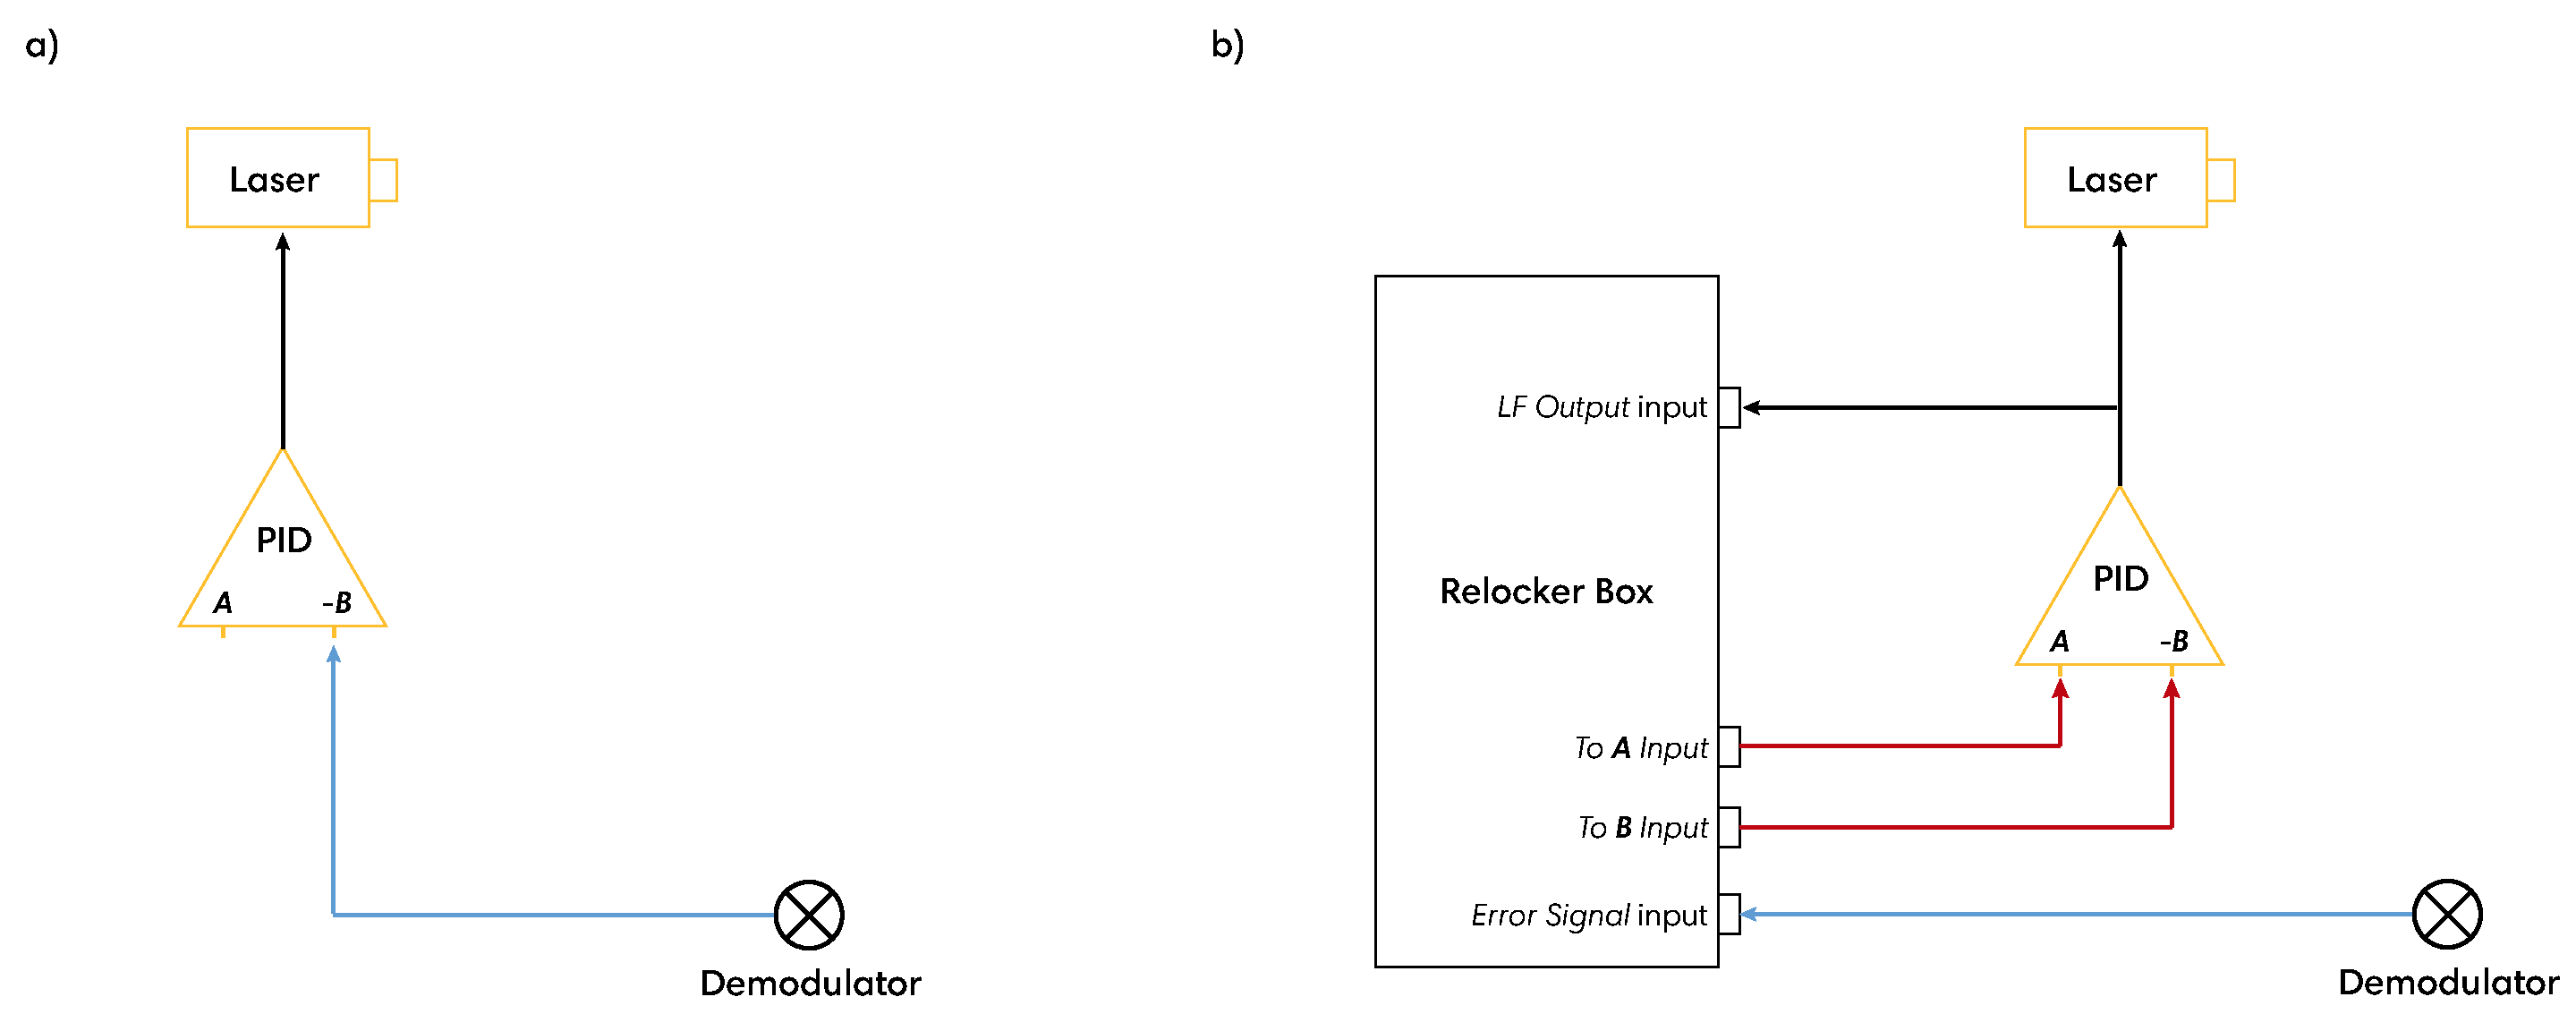
\includegraphics[width=\textwidth]{includes/relockerExtStructure.png}
    \caption{The loop filter stage of a PDH or FM spectroscopy system, \textbf{(a)} before relocker implementation and \textbf{(b)} after relocker implementation.}
    \label{fig:relockerExtStructure}
\end{figure}

Figure~\ref{fig:relockerExtStructure} shows how the relocker box fits into the loop filter stage of the PDH or FM spectroscopy system. In this setup, the relocker box outputs signals to the loop filter's A and -B inputs. 

The box connections serve as the middle man for the three important signals detailed in the previous section. First, the microprocessor's relocking signal runs through the box's ``To A Input'' channel. The box takes in the loop filter's output voltage and the demodulator's error signal, transforming them into a useful format and feeding them to the microprocessor.

\section{Internal Box Connections}
\label{sect:internalBoxConnections}

Figure~\ref{fig:relockerIntStructure} shows the relocker box's internal structure. The shaded elements fall into four main categories: control panel modules, level shifters, buffer amplifiers, and loop filter input switches. Each of these elements enable the microprocessor to perform one of its functions. In all voltage equations, $\text{V}_{\text{Bias}}=5$ V

\subsection{Control Panel Modules}

The simplest category of elements on the diagram is the control panel module category. All such elements are shaded in pink, and extend a knob, switch, or light outside of the box for user interaction.

\begin{itemize}
    \item The ``Mode Indicator LED Circuits'' at the bottom of the microprocessor run four LEDs on the front of the box. Each one illuminates during an important phase of the relocker box's functioning and conveys to the user important information on the cavity-locking system's state. See Table \ref{tab:leds} for LED codes.
    \item The ``Power Supply Switch'' in the top right can be found at the bottom left of the box's front panel. This knob handles the simple On/Off of the box, but if the microprocessor is connected to USB, the microprocessor and LEDs still have power. However, the box will not function without the external power.
    \item The ``Error Signal Sample'' switch above the microprocessor can be found at the bottom right of the control panel. This usually feeds GND into the microprocessor. When it feeds 5 V in, and the code is in the calibration loop, the microprocessor knows to start sampling the error signal maximum voltage.
    \item The ``Relock/Calibrate'' switch sits in the top left of the box's front panel. It also defaults to GND, with the 5 V option engaging the microprocessor's \textit{Calibration} function, whose operation is described in the Operating Guide.
\end{itemize}

Notice that there are switches in the red- and blue-shaded components as well. These are imperative for the components to work properly. The user sets the switches based on the loop filter model in the PDH system in question. They extend knobs directly to the right of the power switch on the control panel. Their function will be described in the following section. These two switches were replaced by one old-school switch, which was hard to find. Any 3P3T switch should have worked.

\subsection{Level Shifters}

The microprocessor communicates with the PDH system via its voltage input and output pins. Since the microprocessor deals in digital information while the PDH deals in analog, conversion between the two formats is crucial for the two systems to cooperate. The microprocessor carries on-board components for this very purpose: analog-to-digital converters (ADCs) and digital-to-analog converters (DACs).

An ADC works by reading the analog voltage on its input pin and assigning a digital level to that voltage. It passes this integer to the main processing chip which can use it in computations. In the relocking system structure shown in Figure~\ref{fig:relocker_structure} \textbf{(b)}, ADCs manage the loop filter output from the PID (black arrow) and the error signal input from the demodulator (blue arrow). In Figure~\ref{fig:relockerIntStructure}, ADCs run on the microprocessor pins \LFOutPin{} and \errMonPin.

A DAC simply works as an ADC in reverse. The main processing chip calculates the digital parameter associated with the voltage it wants to output, then passes this to the DAC managing one of the output pins. The DAC converts this parameter to its analog voltage and outputs the voltage on its pin. In Figure~\ref{fig:relocker_structure} \textbf{(b)}, DACs manage the microprocessor's relocking signal output (orange arrow). These DACs run on microprocessor pins \coarseDACOut{}  and \fineDACOut{}  in Figure~\ref{fig:relockerIntStructure}.

Each converter type uses its own parameter scale. The following table displays each converter's voltage range and the parameters associated with these voltage extremities. Every parameter scale has a step size of one.

\begin{center}
\begin{tabular}{ c||c|c||c|c||c|c }
& \multicolumn{2}{c||}{Correction Signal ADC} & \multicolumn{2}{c||}{Error Signal ADC} & \multicolumn{2}{c}{Relocking Signal DAC} \\
& \multicolumn{2}{c||}{\LFOutADC{} } & \multicolumn{2}{c||}{\errMonADC{} } & \multicolumn{2}{c}{ } \\
& \multicolumn{2}{c||}{\textit{ADC\_DelSig}} & \multicolumn{2}{c||}{\textit{ADC\_SAR}} & \multicolumn{2}{c}{\textit{VDAC8}} \\
\hline
& Voltage & Parameter & Voltage & Parameter & Voltage & Parameter \\
\hline
Low & 0 V & 0 & 0 V & 0 & 0 V & 0 \\
\hline
High & 5 V \textcolor{red}{6.114V?} & 65535 & 2.048 V & 4000 & 4.080 V & 255
\end{tabular}
\end{center}

As is apparent, each converter operates with its own analog voltage range. These ranges do not coincide with the loop filter or demodulator ranges in which they need to operate. For example, common loop filters output a voltage range of $\pm4~\text{V}$, clearly far beyond what the correction signal ADC can convert on its own. Below are the analog voltage ranges in which the feedback system requires the microprocessor to communicate.

\begin{center}
\begin{tabular}{ c||c||c||c }
& Correction Signal Range & Error Signal Range & Relocking Signal Range \\
\hline
Low & -4 V, -11 V, or -14 V & -0.5 V & -4 V, -11 V, or -14 V \\
\hline
High & 4 V, 11 V, or 14 V & 0.5 V & 4 V, 11 V, or 14 V \\
\end{tabular}
\end{center}

The varying voltage lows and highs stem from variations in loop filter construction. JILA loop filters fall into three broad categories: those with outputs ranges of -3.5 V to 3.5 V, -10.5 V to 10.5 V, and -13.5 V to 13.5 V. 

These mismatched range boundaries pose an issue to the microprocessor-PDH interfacing. We need to align the ranges of the converters with the ranges of the signals they convert.

The solution to this problem is level shifting op amp circuitry. Positioned between each converter and its connection to the PDH system is a level shifting circuit which scales and translates the voltage signals into the appropriate range for the recipient. Due to the variation in loop filter output ranges, the circuits must be switchable to the loop filter model in question.

\subsubsection{Loop Filter Output Level Shifter}

First up is the red-shaded level shifter (Fig.~\ref{fig:relockerIntStructure}). The loop filter's output to the cavity controller can span $\pm4$ V, $\pm11$ V, or $\pm14$ V, while the microprocessor's dedicated ADC can only read a signal between 0 V and 5 V \textcolor{red}{6.114V?}. This level shifter scales the loop filter's signal down to a 5 V span, then shifts the zero-point of the signal up to $2.5$ V. The former function lays in the feedback component of the circuit, connected to the inverting op amp input, while the latter lays in the bias component, connected to the non-inverting input. To work with the three possible voltage spans, the circuit needs three gain and bias combinations. We achieve this through the three resistor combinations. The user can choose which combination to use by toggling the rotary switch on the control panel. The op amp's output enters the microprocessor via the \LFOutPin{} once the level shifting is done. This level shifter's output voltage equation is:

\begin{equation}
	\text{V}_{\text{out}}= -\frac{\text{R}_{\text{RFLF}}}{\text{R}_{\text{RSLF}}} \text{V}_{\text{Lp. Fltr. Out}} + \left(1+\frac{\text{R}_{\text{RFLF}}}{\text{R}_{\text{RSLF}}}\right)\left(\frac{\text{R}_{\text{RLLF}}}{\text{R}_{\text{RLLF}}+\text{R}_{\text{RULF}}}\right) \text{V}_{\text{Bias}}.
\end{equation}

\subsubsection{Error Signal Level Shifter \textbf{and} Voltage Limiter}

The PDH system's demodulator output, or the ``error signal'' will usually span between -0.5 V and 0.5 V with a 0 V center point, while the microprocessor's ADC dedicated to the error signal needs a signal between 0 and 2 V. In case the input is above this range, we also include a little diode circuitry to limit the voltage. The level shifting/limiting circuit for this signal is shaded in yellow. It runs on a similar setup as the loop filter output level shifter, with a scaling component contained in the feedback portion of the circuit and a bias component contained in the non-inverting input portion. While the error signal size can vary between setups, the variation should be sufficiently small to require only one resistor combination. The level shifted error signal enters the microprocessor through the \errMonPin. The output voltage equation for the error signal level shifter is:

\begin{equation}
	\text{V}_{\text{out}}= -\frac{\text{R}_{\text{RFES}}}{\text{R}_{\text{RSES}}} \text{V}_{\text{Error Signal}} + \left(1+\frac{\text{R}_{\text{RFES}}}{\text{R}_{\text{RSES}}}\right)\left(\frac{\text{R}_{\text{RLES}}}{\text{R}_{\text{RLES}}+\text{R}_{\text{RUES}}}\right) \text{V}_{\text{Bias}}.
\end{equation}

The voltage limits are set by:

\begin{align}
V_{\text{min}} &= 0\text{ V} = V_{\text{neg. supply}} \frac{R_3}{R_2} - V_\text{diode} \left(1 + \frac{R_3}{R_2}\right)\\
V_{\text{max}} &= 2\text{ V} = V_{\text{pos. supply}} \frac{R_4}{R_5} + V_\text{diode} \left(1 + \frac{R_4}{R_5}\right)
\end{align}

\subsubsection{Microprocessor Output Level Shifter}

To relock the cavity, the microprocessor outputs its voltage sweep through a range preset by its programming. This sweep comes out of the microprocessor in two parts, one from the \coarseDACOut{} {} pin and one from the \fineDACOut{} pin. Each DAC is only 8-bit, (16 mV/bit) which is not very much resolution, so we scale the DACs and sum their signals using the blue-shaded level shifter circuitry. Once again, the microprocessor's operating range does not coincide with the loop filter's range. Here, the microprocessor can only output a signal from 0 V to 4 V, while the necessary signal must be able to span $\pm4$ V, $\pm11$ V, or $\pm14$ V, depending on the loop filter. The level shifter scales and shifts using circuit components comparable to the other two shifters. The adjustability is similar to the red level shifter, with three resistor combinations that offer three gain and bias combinations for converting the microprocessor signal into the range appropriate for the loop filter model in use. Voltage outputs for this circuit obey the equation:

\begin{equation}
	\begin{aligned}
	\text{V}_{\text{out}}=& -\frac{\text{R}_{\text{RFMP}}}{\text{R}_{\text{RSC}}} \text{V}_{\text{Coarse DAC}} -\frac{\text{R}_{\text{RFMP}}}{\text{R}_{\text{RSF}}} \text{V}_{\text{Fine DAC}} + \\
	& \quad \left(1+\frac{\text{R}_{\text{RLMP}}({\text{R}_{\text{RSC}}+\text{R}_{\text{RSF}}})}{\text{R}_{\text{RSC}}\text{R}_{\text{RSF}}}\right)\left(\frac{\text{R}_{\text{RLMP}}}{\text{R}_{\text{RLMP}}+\text{R}_{\text{RUMP}}}\right) \text{V}_{\text{Bias}}
	\end{aligned}	
\end{equation}

This circuit's output enters the A input switch. More on this in Subsection~\ref{subsect:loopFilterInputSwitches}.

Implementing two DACs in this fashion ensures that the voltage sweep is sufficiently fine as to truly scan through the error signal rather than step over it.

To understand this potential problem, consider if a single DAC ran the voltage sweep. Since the DAC can only convert discrete parameters, it can only output discrete voltages. When the microprocessor tries to sweep using this DAC, the best it could do is set the DAC voltage at one parameter level, then recursively step the parameter up over time. The result is a granular sweep with discrete voltage ``steps'' rather than a continuous ramp. This poses a problem to the microprocessor's ability to relock. As stated earlier, the microprocessor looks for the error signal profile while it sweeps to identify when the cavity is back in lock. If the sweeping step size is large enough that it spans the voltage width of an error signal profile, the microprocessor risks stepping over the profile. Figure~\ref{fig:esig_jumpover} illustrates this possibility with sample DAC parameters.

\begin{figure}[h!]
	\includegraphics[scale=.35]{includes/esig_jumpover}
	\centering
	\caption{An illustration of the DAC's sweep stepping over the error signal. The bar underneath the plot depicts the voltage widths of each DAC step. The step width could, as in this figure, span the entire width of the error signal.}
	\label{fig:esig_jumpover}
\end{figure}

Because the microprocessor's code only allows a single function per clock cycle (i.e. it can either step up the sweep, or check for the error signal, but not both at the same time), it would step over the profile when jumping from parameter 100 to 101, \textit{then} check for the profile. It would thus fail to see the profile and subsequently fail to re-engage the PID controller on time.

The remedy to this issue is to employ two DACs for sweeping the voltage: a coarse DAC output and a fine DAC output. We set the coarse DAC's total range to coincide with the PID controller's total range while we set the fine DAC's total range to span one step size of the coarse DAC. The resistors RSC and RSF accomplish this scaling.

To sweep the voltage under this model, we set the coarse DAC's output to one parameter, then sweep the fine DAC's output through its entire range. This sweeps the combined output through the original DAC's single-step span. When the fine DAC reaches its limit, we step the coarse DAC up one parameter, then reset the fine DAC to zero for its next fine sweep. Figure~\ref{fig:esig_njumpover} depicts this DAC range configuration.

\begin{figure}[h!]
	\includegraphics[scale=.35]{includes/esig_njumpover}
	\centering
	\caption{The fine DAC's full range fits inside the coarse DAC's single-step range.}
	\label{fig:esig_njumpover}
\end{figure}

By this method, the microprocessor can sweep through the previously unreachable intermediate voltages. It can output a more continuous sweep to the PID and observe the error signal response in finer detail, ensuring that it does not jump over the profile it seeks.

Upon powering, the microcontroller determines if the loop filter range knob has selected `8V', `22V', or `28V' (\texttt{LFRange}). This setting determines where the 150mV threshold for detecting an unlocked signal lies. This setting is not changed while the box is running.

\subsection{Buffer Amplifiers}

The microprocessor's ability to output current is relatively low, resulting in possible drops in voltage when the blue level shifter sources too much current (Op amps of coarse have high impedances, which is why this phenomenon perplexes me; it would seem that such a current loading problem should not occur, but it does, hence the buffer amplifiers. Perhaps you can figure out why the problem occurs when the microprocessor tries to output to the level shifter?). The buffer amplifiers shaded in orange serve to prevent unchecked current sourcing, keeping the microprocessor's output voltage true.

\subsection{Loop Filter Input Switches}
\label{subsect:loopFilterInputSwitches}

The microprocessor switches the loop filter between its conventional functioning and following mode by switching the inputs to the loop filter. Enabling this control are the two green-shaded switches. One feeds its common channel into the loop filter's A input while the other feeds its common channel into the loop filter's -B input. They are SPDT switches chosen such that they can pass along signals ranging between $\pm15$ V (primarily this meant finding MAX319CPA switches that could run on $\pm15$ V power rails).

Important to note is how they configure their disengaged throws. When one throw is connected, the other is left hanging, detached from anything. A switch configured to do this is known as a reflective switch, in contrast with an absorptive switch, which connects its disengaged throw to a resistor to ground. A reflective switch is crucial to use in the relocker box because it keeps the disengaged signal at its true voltage. If there was a resistor connecting it to ground when it was disengaged (the absorptive type operation), a voltage divider could form, raising the signal's voltage in magnitude for the duration of disengagement, and the microprocessor would read in a false voltage. Such false voltage readings skew the microprocessor's code parameters and cause relocking attempts to fault.

The A switch options are, as shown in Figure~\ref{fig:relocker_structure}(b) for the A input of the loop filter, GND and the relocking signal from the microcontroller after level shifting. GND takes the NC (Normally Closed) terminal of the switch as the resting state of the loop filter should be in its conventional PDH configuration. Only when the microprocessor switches the switch control terminal to high via its \aPin{} pin does the switch engage the NO (Normally Open) option, the relocking signal.

The B switch options of course correspond to the Figure~\ref{fig:relocker_structure}(b) options for the -B input of the loop filter. The demodulator's error signal takes the NC terminal as per conventional PDH setups, while the loop filter's own unmodified output connects to the NO terminal. When the latter engages, the loop filter's following mode comes into effect. 


\subsection{``Triggered'' Relocking (Block Lock TTL)}\label{subsec:blockLock}
There may be experiments where a lock is intentionally dropped, and the box needs to wait for a trigger before attempting to relock. For example, we may turn off the lattice laser, causing the lock to the cavity to drop; after the trial, the laser can be turned on and relocked for the next trial.

The relocking function can be stopped by using the Block Lock TTL (\blockLockPin{}). When the pin is left low, relocking is permitted as usual, and when the pin is high, the code loops uselessly until the pin goes low again.

\begin{figure}[h]
    \centering
    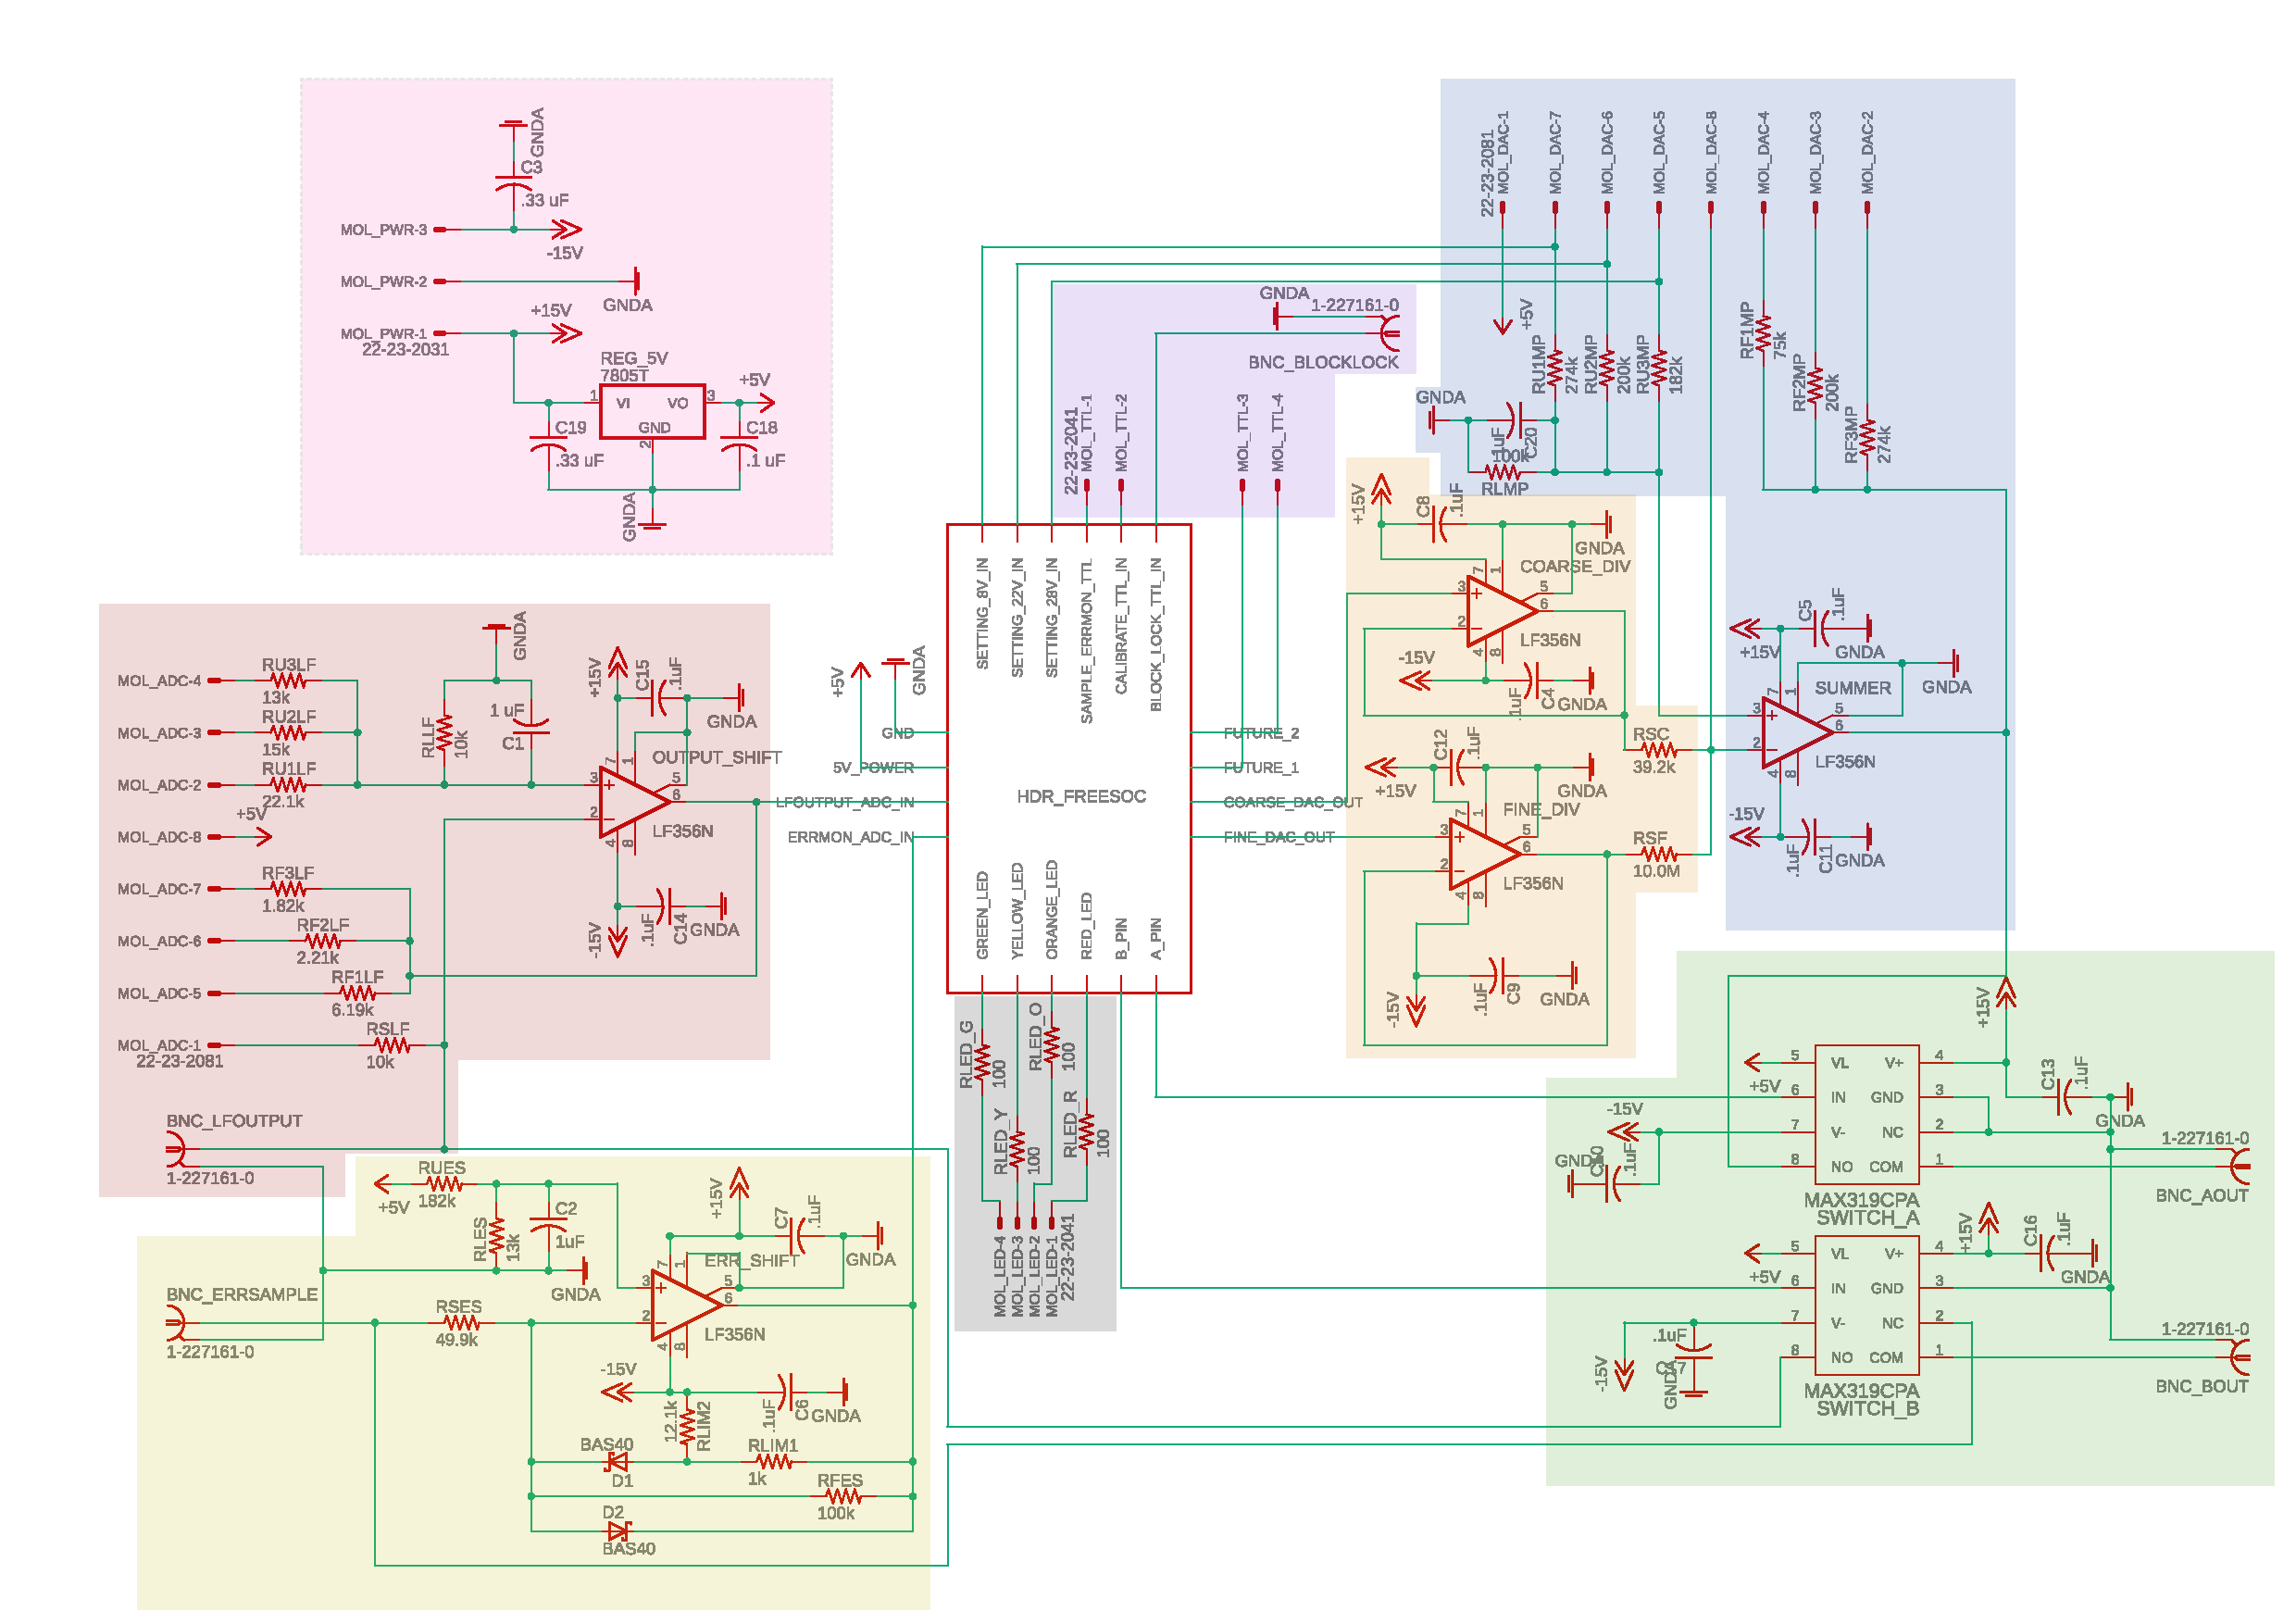
\includegraphics[width=1.0\textwidth,angle=90]{includes/relocker_pcb_schematic_colored.pdf}
    \caption{The internal structure of the relocker box.}
    \label{fig:relockerIntStructure}
\end{figure}

\chapter{Relocker Algorithm}\label{chap:relockerAlgorithm}

Here we examine the microprocessor algorithm itself. We first study the board components employed in the relocker algorithm, then the pin assignments, and finally the code. For a brief introduction to the relocker's microprocessor, the FreeSoC2 development board, consult the Appendix. PSoC Creator 4.0+ was used.

\begin{figure}[h]
    \centering
    \includegraphics[width=0.75\columnwidth]{includes/relockerTopDesign.png}
    \caption{The top design of the code. Here we implement the onboard components we will use in the code.}
    \label{fig:relockerTopDesign}
\end{figure}

Figure~\ref{fig:relockerTopDesign} shows the top design of the code. This is the first panel to set up when programming the microprocessor. This is where we implement board components.

We use two ADCs. The ADC for the loop filter signal conversion is a delta-sigma ADC. It reads in its signal from the \LFOutPin, whose voltage is the level shifted loop filter output. This ADC runs with 16-bit resolution in single-ended mode (no differential inputs), with valid input voltages from 0 V to 6.144 V. We scale the loop filter's voltage span down to 5 V because in fact the microprocessor's pins can only handle up to 5.5 V. The successive approximation register (SAR) ADC reads in the level shifted error signal from the \errMonPin. The conversion resolution runs at 12 bits, and operates in single-ended mode with a voltage range of 0 V to 2.048 V.

Each voltage DAC manages one of the microprocessor's outputs. As stated earlier, one outputs the coarse voltage sweep while one outputs the fine voltage sweep. Both operate in the 0 V to 4.080 V range. Their outputs connect to the microprocessor output level shifter as shown in Figure~\ref{fig:relockerIntStructure}.

The control register manages the voltage on the \aPin{}  and \bPin{}  pins. They are tied together due to their function: the \aPin{}  and \bPin{}  switch the loop filter between being controlled normally and by the microcontroller. If one pin lags behind the other, patchy switching or signaling can occur, hence the setup for simultaneity in voltage switching achieved through wiring them all to the control register. When switching is in order, the microprocessor need only switch the voltage on the register and all connected pins will switch together. (In fact, we could have wired the orange light, A switch, and -B switch controls all to one pin to achieve simultaneity. This is but one solution.) Finally, the rest of the pins implemented on the board lay arranged under the control register.

Notice that some of the pins connect to components right on the top design while some are free floating. The user can configure the pins to operate in either mode. As one would expect, the code cannot directly write to the output pins connected to the DACs in the top design--in order to change the voltage output on these pins, the code needs to write to the associated DACs which then pass along the directive. The code can, however, write directly to the free floating pins. These pins take direction straight from the CPU, and thus act as the processor's easiest means for digital signal reading and writing.

\begin{figure}[h]
    \centering
    \includegraphics[width=\textwidth]{includes/relockerPinAssignments.png}
    \caption{Pin assignments on the board}
    \label{fig:relockerPinAssignments}
\end{figure}

After implementing all of the pins in the top design, the user must assign those pins to physical pins on the edge of the microprocessor chip using the \texttt{.cydwr} file tab in the programming IDE, shown in Figure~\ref{fig:relockerPinAssignments}. It is an unfortunate circumstance that both these components share a name. To clarify, there are indeed two ``types'' of pins. There are the CPU's pins, shown on the CPU schematic in Figure~\ref{fig:relockerPinAssignments}. Their number assignments on the CPU chip are set in stone. When we implement pins into the top design, they are not yet associated with a physical CPU pin. It is in this tab that we associate them. The IDE will automatically choose a CPU pin for the pin in question unless the user overrides that choice and chooses a different pin. The user \textit{should} do this using the right side column labeled ``Pin''. Choosing pins for specific purposes is sometimes in order as certain CPU pins exhibit special capabilities that allow them to perform certain functions better than others. 

At the same time, there are pins on the periphery of the microprocessor board. These pins are divided into ``ports'' on the board, which are essentially groups of pins. When referring to these board pins, we call them by their port, then their pin number. For example, the \aPin{}  is wired to pin P12[3], or ``port 12, pin 3''. Once a top design pin connects to a CPU pin, that CPU pin needs to connect to a peripheral board pin as the board pin is what interacts with the external world. Board pins also have specialized capabilities that make selecting board pins an important practice. The user can choose the board pin with which the CPU pin connects using the column on the right labeled ``Port''.

\section{Calculating Voltage Sweep Bounds}

The C++ procedure for calculating voltage sweep bounds is quite involved (lines 146 through 186). This section provides a simple overview using the Figure~\ref{fig:voltageSweepDiagram}.

\begin{figure}[hbt]
    \centering
    \includegraphics[scale=0.5]{includes/voltageSweepDiagram.png}
    \caption{...}
    \label{fig:voltageSweepDiagram}
\end{figure}

Consider a PDH system running with a loop filter whose output spans -4 V to 4 V. There will be a cavity lock voltage somewhere within those bounds, shown on the diagram in red. As stated in the code comments, the microprocessor needs to set voltage bounds around that lock voltage. These are shown in green, at $\pm$150 mV. (In every loop filter voltage range, these bounds correspond to different digital levels. Error signals wander within this range, never beyond, so it works well as the ``out of lock'' threshold.) Although the parameter scaling of the ADC and DACs do not coincide, their full range still corresponds with that same -4 V to 4 V span. Thus, we can align their scales as shown in the diagram, knowing that the lock voltage proportionally scales onto the ADC and DAC bars. On the DAC bar, we are showing the coarse DAC step sizes in grey. These are not to scale of course; in reality, there would be 255, but for the purposes of this illustration, we have shown them zoomed in.

There are two parameters that matter in the DAC bar: the \coarseDAC{}  parameter and the \fineDAC{}  parameter. These are shown as pairs on the diagram, with the first number being the \coarseDAC{}  parameter. Once the \LFOutADC{}  has read in the lock voltage in terms of the ADC parameter, the code uses that parameter to calculate the DAC parameter pair that corresponds to that voltage. This means calculating the \coarseDAC{}  parameter just shy of the correct voltage, then calculating the \fineDAC{}  parameter that fills in the remaining change. Conversion ratios between the ADC parameters and the DAC parameters are key for this calculation. It then calculates the DAC parameter pairs of the upper and lower sweep bounds. These bounds can end up scattered between coarse DAC steps, as shown in the DAC bar.

No worries, we know how to use binary numbers. Treat the sweep voltage as a single 16-bit number, \texttt{sweepV}. The least significant 8 bits are for \fineDAC{} , and the most significant 8 bits are for \coarseDAC{} . Then we just need to count \texttt{sweepV} from the lower to upper bounds, outputting \texttt{(0xff00 \& sweepV >> 8)} and \texttt{(0x00ff \& sweepV)} to \coarseDAC{}  and \fineDAC{}  respectively.



If the need ever arises to understand Denton's old DAC sweep parameters, a table of parameter settings can be found in the ``Denton's Relocker'' OneNote. Look for the note entitled ``2 Nov 2017: Once and for all: Setting down the voltage sweep parameter bounds''. Here you'll find a list that details the voltage bounds in terms of the DAC parameters. It was this list that he translated into the code, but this method is not used anymore.

\section{The Code}

\begin{spacing}{1.0}
\lstinputlisting{"../src/Adjustable Automated Relocker Code/Adjustable Automated Relocker Code.cydsn/main.c"}
\end{spacing}


\section{Calibrating the Voltage Sweeps}
As discussed, the voltages the microprocessor can read and write are different from the voltages that interact with the loop filter. It is useful to have internal functions that can transform between the two, but this requires 30 minute calibration. I expect this calibration only needs to be recorded once for new resistor values. The software has been left behind in an auxiliary \texttt{calibration.c} file, and the physical procedure is as follows. Note that offsets should be done first, and all values are set near the part of the code that determines which loop filter setting is active.
\begin{enumerate}
	\item Connect to and run the serial communications program (Chap.~\ref{chap:serialcomm}).
	\item Set \texttt{TEXT\_VOLTAGE\_MODE=true}. This enables a subroutine that sweeps the DACs and measures the ADCs. LEDs should be blinking two at a time, in an alternating manner.
	\item \begin{enumerate}
		\item Attempt to output 0V out of the \textit{A output} with \texttt{DAC\_VoltsTo\_Counts(0.0, float DACRange, int DACOffset)} and correct the \texttt{DACOffset} variable for each of the \texttt{LFRange} settings until you see true 0V output.
	\item Attempt to output 1V with \texttt{DAC\_VoltsTo\_Counts(1.0, float DACRange, int DACOffset)} and correct the \texttt{DACRange} variable for each of the \texttt{LFRange} settings until you see true 1.0V output.
	\item Verify the 0-1V and full range sawtooth waves in the calibration subroutine look good out of the A output.
	\item Repeat for each \texttt{LFRange}: 8V, 22V, 28V.
	\end{enumerate}
	\item Ground the error signal input and use the calibration subroutine to measure the DAC value of the error monitor signal. This becomes the global \texttt{errMonADC\_SetOffset(\textit{\textit{meas}})}. I measured 1992.
	\item Put a known voltage approximately 0.4V in the error signal input and scale \texttt{errorMonADC\_SetGain(\textit{value})} until the reading is correct. I measured -3982. Note the error monitor calibration is independent of the loop filter range.
	\item Repeat this procedure for the 8V, 22V, and 28V range Loop Filter Output ADC offsets and gains.
\end{enumerate}


\chapter{Known Issues and Future Work}
\label{chap:knownIssuesAndFutureWork}

Here I'll run through known issues in the system and some solutions that I've found work well. The reader interested in advancing the system should take these issues as starting points for improvement.

\section{Cleaning up the Error Signal}
\label{sec:cleaningUpTheErrorSignal}

Certain error signals can be extremely noisy, and as a result, pose a difficult challenge to the microprocessor which works best with clean error signals. 

The reason for this behavior lies in the code's process for relocking. As shown earlier, the microprocessor only relocks when it sees that the error signal has passed beyond the detection threshold and then passed back in. Clean error signals pass the threshold in a crisp and unambiguous fashion. Noisy signals do not; their voltage jitter can be quick and large enough that when the microprocessor is pulling the signal back to its center-point zero and the signal is about to make its first pass over the threshold, the voltage noise can jump past the threshold and back before the error signal has made its true pass. This quick phenomenon trips the microprocessor's detection code, cuing it to switch the system back to conventional PDH setup before the error signal has entered its central linear region in earnest.

Cleaning up the error signal is thus in order. I've found that installing a low pass filter on the error signal line helps with this ``false-relock'' phenomenon. That is not to say that it's a complete solution. Certain problems arise as a result of installing the filter. Primarily, the filter will also attenuate the error signal itself, something that becomes increasingly noticeable as the user ramps up the relocking sweep speed. It also becomes hard to see the true error signal when the dither is on because of this attenuation. If the researcher is not concerned with these issues, the low pass filter is fine; he or she should simply make sure to install the low pass filter while setting up the error signal component of the relocker. If the researcher is concerned with these issues, I believe approaching a solution to the false-relock phenomenon from a coding perspective would be the way to go.

There are two possible solutions in my mind as of now. A simple one would be to program a delay into the detection threshold double-pass code. This would instruct the microprocessor to wait just a few microseconds before looking for the second pass of the error signal, thereby directing it to ignore noise fluctuations that could mimic the second pass. The user might have to gauge the frequeny of the noise to find exactly how long the delay should be. The second solution (a Graham idea) is to program an averaging function into the error signal read-in. This code would take the past, say, five error signal readings and average them to ``unweight'' the noise and find a truer reading on the error signal value. Running this every read-in cycle would give the microprocessor real-time updates on the true error signal that are less affected by noise.

\section{Offsetting the Center of the Voltage Sweep}

At one point, Denton offset the \texttt{sweepCenter} variable by a few DAC steps. This offset was there to compensate for imprecisions in coinciding the full DAC range with the full loop filter output range. Ideally these ranges would be perfectly adjusted by the level-shifters such that their center and ranges match exactly. This is rarely the case, hence the necessity for offsetting the DAC just a bit. The easiest way to do this is in the code; it can take some trial and error to find exactly how far to offset the \texttt{sweepCenter} variable.

Making the circuits more precise would rid the code of the necessity to compensate for imprecision in level-shifting. Using fine-tunable potentiometers would be one option; these would take the place of the code offset. Providing a potentiometer knob on the outside of the box would allow for great tunability with easy access. It would also introduce user error.

\section{Slowing Down the Relocking Sweep}

Error signals can vary quite a bit in size and shape. If the user is dealing with a signal that's narrow, the relocking signal may sweep through the center of the error signal faster than the microprocessor can detect for threshold-crossing. The remedy is to slow down the relocking sweep. The way to do this is using delays in the program. I've already programmed into each voltage sweep loop a delay statement; for every pass through the loop, the microprocessor will wait when it encounters these statements, and then proceed. The time delay is set by the parameter inside the delay command. Useful for us are the delay commands \texttt{CyDelay(x)} which instructs the microprocessor to wait $x$ milliseconds after each voltage step, and \texttt{CyDelayUs(y)}, which instructs the microprocessor to wait $y$ microseconds after each step. By trial and error, the user can choose longer or shorter delay times to get the optimal relocking sweep speed for the system at hand.




%%%%%%%%%%%%%%%%%%%%%%%%%%%%%%%%%%%%%%%%%%%%%%%%%%%%
%      Chapter Eight: Serial Communication         %
%%%%%%%%%%%%%%%%%%%%%%%%%%%%%%%%%%%%%%%%%%%%%%%%%%%%
\chapter{Serial Communication}\label{chap:serialcomm}

Serial communication can be very powerful for debugging or for transferring information to and from the microprocessor. This chapter includes notes on sending commands and data from the relocker box, to a computer, through a USB cable. It also details the ``Serial Communications Server'' program written in Python.


\section{Serial Communications Server}
\label{sect:serial_comm_server}
\subsubsection{Dependencies}
This program will only work for Windows 7+ and Python 3+. Further, \texttt{pyserial} and \texttt{colorama} must be installed through websites or by running the following commands:
\begin{lstlisting}
python -m pip install pyserial
python -m pip install colorama
\end{lstlisting}

\subsubsection{Using the Program}
First, the microcontroller's ``Debugger'' microUSB port should be connected to a computer USB port. Run the program as you would run any Python script:
\begin{lstlisting}
python relocker_serial_comm.py
\end{lstlisting}
and you should see a list of accessible COM ports (USB connections). Enter the port number and the program will begin listening for any data transmitted by the microcontroller. If no COM ports are available, verify that they are visible in Device Manager, or try listening to the transmitted signals through a serial port reader such as Tera Term or PuTTY. If the port is there but inaccessible, try re-powering the box or pressing the \textit{Debugger Reset} switch on the FreeSoc board.

When programming the microcontroller, use documentation for \texttt{SW\_Tx\_UART} or the provided \texttt{Serial()} macro to send bytestrings to the Python program. The ``Debugger'' port Tx seems to be hardwired to \texttt{P2.1}, which I found out through the SparkFun pinout diagram (see Sec.~\ref{app:resources} in the Appendix). The Baud rate (and other settings such as parity bit which don't seem accessible through the software UART), for the UART and Python serial port should be set the same. I chose the maximum of 115200/s.
	
\textbf{For new projects, a note on printing floating point}: printing floats with \texttt{sprintf()} turned out to be a big pain. The compiler/linker avoids including this functionality unless \texttt{Use newlib-nano Float Formatting} is set to \textit{True} in \texttt{Project > Build Settings > ARM GCC 5.4... > Linker}. There is also a memory issue, so select the \texttt{.cydwr} file's tab along the top and the \texttt{System} tab along the bottom; then change \textit{Heap Size (bytes)} from 0x80 to 0x0200.




%%%%%%%%%%%%%%%%%%%%%%%%%%%%%%%%%%%%%%%%%%%%%%%%%%%%
%      Chapter Nine: Printed Circuit Board         %
%%%%%%%%%%%%%%%%%%%%%%%%%%%%%%%%%%%%%%%%%%%%%%%%%%%%
\chapter{Printed Circuit Board}\label{chap:pcb}

A PCB was used to make this design a little more robust, and to assist if this is actually useful. The schematics and board layout were drawn in EAGLE. I used a variety of tutorials to remember how to use EAGLE, but the \href{https://learn.sparkfun.com/tutorials/using-eagle-schematic}{SparkFun EAGLE tutorials} were particularly helpful. I tried to leave room for additional circuitry if it becomes necessary, but I also aimed for a compact layout. After generating the Gerber files with the SparkFun CAM job file (see their tutorial part 2, but I don't think the generation details are important), we printed the boards with PCB Unlimited's panel-share economy pricing. It takes 10 days but the cost per square inch is just over a dollar. There are cheaper alternatives but this is clearly a high quality board.

I made a custom library and device for the header to the microprocessor, and I had to use a program called Universal Library to import the MAX319 switch IC. It would have been fine to use a generic DIP package but this kept the pin labeling from the manufacturer. Some layout suggestions from across the internet: keep bypass capacitors between a voltage source and an IC pin; keep resistors close to the high-impedance inverting input of op amps; and insert ground planes early on in the layout. I also left an extra pin, and the Block Lock / Sample Hold BNCs can potentially be reconfigured to share an input.

The first iteration of the board layout is shown in Fig.~\ref{fig:pcblayout}.

\begin{figure}[hbt]
	\centering
	\includegraphics[width=.75\textwidth]{includes/relocker_pcb_layout.pdf}
	\caption{PCB Layout}
	\label{fig:pcblayout}
\end{figure}

\bibliographystyle{unsrt}
\bibliography{relocker_bibliography}

\begin{appendices}

\section{Pictures of the Relocker Box, as of June 15, 2018}

\begin{figure}[H]
    \centering
    \includegraphics[width=0.5\columnwidth]{includes/relockerFront.jpg}
    \caption{Front of the relocker, showing the control panel.}
    \label{fig:relockerFront}
\end{figure}

\begin{figure}[H]
    \centering
    \includegraphics[width=0.5\columnwidth]{includes/relockerBack.jpg}
    \caption{Back of relocker, showing connections.}
    \label{fig:relockerBack}
\end{figure}

\begin{figure}[H]
    \centering
	\includegraphics[width=0.5\columnwidth]{includes/relockerInterior.jpg}
    \caption{The relocker's interior.}
    \label{fig:relockerInterior}
\end{figure}

\section{Notes on the Microprocessor}\label{app:resources}

The microprocessor I've used in this project is Sparkfun's FreeSoC2 development board. It costs about \$50, and runs on Cypress's PSoC 5LP microcontroller. The IDE for programming the device is the PSoC creator whose three parts I displayed earlier.

Some interesting features of the IDE are the PSoC creator's use of the schematic as a way to implement components on the board. Rather than calling on the user to implement components in the main code, the user can implement them by simply dragging components from the components bank onto the schematic. The bank contains every usable tool on the board, including op amps, ADCs and DACs, plenty of GPIO pins, a UART, counters, timers, and more. The bank even contains logic gates that the board can implement so that if the code you're looking to upload is simple enough, you can build it with just a clever schematic.

Each of the components boasts an impressive array of adjustable settings and an API. To aid in usability, Cypress has documented these features through extensive data sheets for every component. These sheets are extremely informative, and offer an excellent starting point for devising the component makeup of a program. They describe all modes of operation in which the user can configure components as well as details on all API programs. 

To access the data sheet as well as configuration controls for a component, simply double-click the component on the schematic. This pulls up the control window for that component, which contains a data sheet link as well as setting switches.

Overall, the FreeSoC2's comprehensive and flexible array of tools make it a superb choice for electronic control in the lab. There really is a great span of projects one can approach with this versatile board, of which a relocker is only one. If you're interested in applying the board for another project, use these links to get started.
\begin{itemize}
    \item Sparkfun's FreeSoC2 product page: \url{https://www.sparkfun.com/products/13714}.
    
    This contains some useful cursory information on the board.
    
    \item A complete first-steps tutorial on programming the FreeSoC2 using Cypress's PSoC Creator: \\
    \href{https://learn.sparkfun.com/tutorials/freesoc2-hookup-guide-v14?_ga=2.8215090.1292973380.1530714260-313202448.1431455612}{\underline{SparkFun Hookup Guide V14}}.
    
    This tutorial runs through the components on the board itself and how to get your first PSoC Creator program working. This is the best place to start! The walkthrough also includes how to run Arduino code on a FreeSoC board.
    
    \item Cypress's PSoC 5LP chip product page: \href{http://www.cypress.com/products/32-bit-arm-cortex-m3-psoc-5lp}{\underline{chip link}}.
    
    Here's where you can download the PSoC Creator IDE and read an overview of the chip's capabilities. This site also links to almost all of the data sheets and technical documentation you'll need on the chip. It's a great resource.
    
    \item The PSoC 5LP chip data sheet: \url{http://www.cypress.com/file/45906/download}.
    
    A bunch of useful, detailed information on the chip. This will give you technical details on the features.
    
    \item The Cypress developer community: \url{https://community.cypress.com/welcome}.
    
    This site holds a fairly active, useful forum.
\end{itemize}




\end{appendices}



\end{document}